\documentclass[12pt]{article}

\usepackage{amsmath}
\usepackage{amssymb}
\usepackage{physics}
\usepackage{enumitem}
\usepackage{tikz}
\usetikzlibrary{arrows.meta,calc,angles,quotes,decorations.pathmorphing}
\usepackage{geometry}
\geometry{margin=1in}

\begin{document}

\begin{center}
\Large \textbf{ULTRA-HARD Physics Paper (JEE Advanced Level)}
\end{center}

%--------------------------------------------------
%--------------------------------------------------
\textbf{Q1.}  
A particle is projected from the surface of the Earth with speed $u$ at an angle $\theta$ with the horizontal.  
The gravitational acceleration varies with height as  
\[
g(h)=g_0\left(1-\frac{2h}{R}\right),
\]
where $R$ is the radius of the Earth and $h \ll R$ throughout the motion.  

Assume that the motion remains confined to heights much smaller than $R$, and treat the variation of $g$ as a small perturbation about uniform gravity.  

To first order in the small parameter  
\[
\frac{u^2\sin^2\theta}{g_0R},
\]
determine the time of flight of the projectile.

\begin{enumerate}[label=(\Alph*)]
\item $\displaystyle \frac{2u\sin\theta}{g_0}
\left(1+\frac{u^2\sin^2\theta}{2g_0R}\right)$

\item $\displaystyle \frac{2u\sin\theta}{g_0}
\left(1-\frac{u^2\sin^2\theta}{2g_0R}\right)$

\item $\displaystyle \frac{2u\sin\theta}{g_0}
\left(1-\frac{u^2\sin^2\theta}{g_0R}\right)$

\item $\displaystyle \frac{2u\sin\theta}{g_0}$
\end{enumerate}
%--------------------------------------------------
\textbf{Q2.}  
A uniform rod (mass $m$, length $L$) is hinged at one end and released from horizontal.  
Find angular speed when rod makes $30^\circ$ with vertical.

\begin{center}
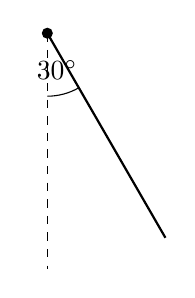
\begin{tikzpicture}[scale=1]
\coordinate (O) at (0,0);
\coordinate (V) at (0,-3);
\coordinate (P) at ({3*sin(30)},{-3*cos(30)});
\fill (O) circle(2pt);
\draw[dashed] (O)--(V);
\draw[thick] (O)--(P);
\draw pic [draw=black, angle radius=0.8cm, "$30^\circ$"] 
{angle = V--O--P};
\end{tikzpicture}
\end{center}

\begin{enumerate}[label=(\Alph*)]
\item $\displaystyle \sqrt{\frac{3g}{L}\left(1-\frac{\sqrt{3}}{2}\right)}$
\item $\displaystyle \sqrt{\frac{3g}{2L}}$
\item $\displaystyle \sqrt{\frac{g}{L}}$
\item $\displaystyle \sqrt{\frac{9g}{8L}}$
\end{enumerate}

%--------------------------------------------------
\textbf{Q3.}  
A block of mass $m$ slides without friction down a wedge of mass $M$ placed on a smooth floor.  
Released from height $h$, the speed of the block relative to ground at bottom is:

\begin{center}
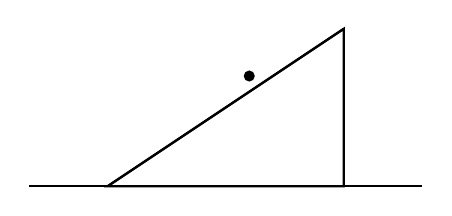
\begin{tikzpicture}[scale=1]
\draw[thick] (0,0)--(5,0);
\draw[thick] (1,0)--(4,0)--(4,2)--cycle;
\draw[thick] (1,0)--(4,2);
\fill (2.8,1.4) circle(2pt);
\end{tikzpicture}
\end{center}

\begin{enumerate}[label=(\Alph*)]
\item $\displaystyle \sqrt{2gh}$
\item $\displaystyle \sqrt{\frac{2ghM}{M+m}}$
\item $\displaystyle \sqrt{\frac{2gh(M+m)}{M}}$
\item $\displaystyle \sqrt{\frac{2ghM}{M+2m}}$
\end{enumerate}

%--------------------------------------------------
\textbf{Q4.}  
Two identical capacitors $C$ in series are connected to battery $V$.  
A dielectric (constant $k$) is slowly inserted fully in one capacitor.  
Heat produced in circuit equals:

\begin{enumerate}[label=(\Alph*)]
\item $\displaystyle \frac{CV^2}{8}(k-1)$
\item $\displaystyle \frac{CV^2}{4}(k-1)$
\item $\displaystyle \frac{CV^2}{4}\!\left(1-\frac{1}{k}\right)$
\item $\displaystyle \frac{CV^2}{8}\!\left(1-\frac{1}{k}\right)$
\end{enumerate}

%--------------------------------------------------
\textbf{Q5.}  
A charged particle enters uniform magnetic field $\vec B$ with speed $v$ making angle $\theta$ with $\vec B$.  
After one complete revolution of its transverse motion, the net displacement magnitude is:

\begin{center}
\begin{tikzpicture}
\coordinate (O) at (0,0);
\coordinate (B) at (4,0);
\coordinate (V) at (2,2);
\draw[->] (O)--(B) node[right]{$\vec B$};
\draw[->] (O)--(V) node[right]{$\vec v$};
\draw pic [draw=black, angle radius=0.8cm, "$\theta$"] 
{angle = B--O--V};
\end{tikzpicture}
\end{center}

\begin{enumerate}[label=(\Alph*)]
\item $0$
\item $\displaystyle \frac{2\pi m v\cos\theta}{qB}$
\item $\displaystyle \frac{2\pi m v\sin\theta}{qB}$
\item $\displaystyle \frac{\pi m v\cos\theta}{qB}$
\end{enumerate}

%--------------------------------------------------
%--------------------------------------------------
\textbf{Q6.}  
One mole of an ideal gas undergoes a cyclic process in the $PV$-plane forming a triangle with vertices  
$(P_0,V_0)$, $(2P_0,V_0)$ and $(2P_0,2V_0)$.  

The cycle is traversed in the order  
\[
(P_0,V_0) \rightarrow (2P_0,V_0) \rightarrow (2P_0,2V_0) \rightarrow (P_0,V_0),
\]
and the gas returns to its initial state.  

Assuming ideal gas behaviour and neglecting heat losses, determine the efficiency of the cycle.

\begin{enumerate}[label=(\Alph*)]
\item $\dfrac{1}{6}$
\item $\dfrac{1}{5}$
\item $\dfrac{1}{4}$
\item $\dfrac{1}{3}$
\end{enumerate}
%--------------------------------------------------
\textbf{Q7.}  
A solid sphere (radius $r$) rolls without slipping inside a spherical bowl of radius $R$.  
For small oscillations about the lowest point, angular frequency is:

\begin{enumerate}[label=(\Alph*)]
\item $\displaystyle \sqrt{\frac{5g}{7(R-r)}}$
\item $\displaystyle \sqrt{\frac{7g}{5(R-r)}}$
\item $\displaystyle \sqrt{\frac{g}{R-r}}$
\item $\displaystyle \sqrt{\frac{2g}{5(R-r)}}$
\end{enumerate}

%--------------------------------------------------
\textbf{Q8.}  
A conducting sphere of charge $+Q$ is surrounded by a neutral conducting shell.  
The shell is grounded and then ground connection is removed.  
Final charge on the outer surface of shell is:

\begin{enumerate}[label=(\Alph*)]
\item $0$
\item $-Q$
\item $+Q$
\item $-\dfrac{Q}{2}$
\end{enumerate}

%--------------------------------------------------
\textbf{Q9.}  
A glass slab (refractive index $n$) of thickness $t$ moves with speed $u \ll c$ parallel to its surface.  
A ray enters normally in the laboratory frame.  
Angle of emergence in laboratory frame (to first order in $u/c$) is:

\begin{enumerate}[label=(\Alph*)]
\item $0$
\item $\displaystyle \frac{u}{c}\!\left(1-\frac{1}{n^2}\right)$
\item $\displaystyle \frac{u}{c}(n-1)$
\item $\displaystyle \frac{nu}{c}$
\end{enumerate}

%--------------------------------------------------
%--------------------------------------------------
\textbf{Q10.}  
Two infinitely long parallel wires are separated by a distance $2d$ and carry equal steady currents $I$ in the same direction.  

A small square conducting loop of side $a$ ($a \ll d$) carrying current $I$ is placed midway between the two wires such that:

\begin{itemize}
\item The plane of the loop is the same as the plane containing the wires,
\item Two sides of the loop are parallel to the wires,
\item The centre of the loop lies on the perpendicular bisector of the line joining the wires.
\end{itemize}

The loop is displaced by a small distance $x \ll d$ toward one of the wires while remaining parallel to its original orientation.

Using first-order approximation in $\frac{x}{d}$ and $\frac{a}{d}$, determine the magnitude of the net magnetic force on the loop.

\begin{enumerate}[label=(\Alph*)]
\item $\displaystyle \frac{\mu_0 I^2 a^2}{\pi d^3}\, x$

\item $\displaystyle \frac{\mu_0 I^2 a^2}{2\pi d^3}\, x$

\item $\displaystyle \frac{\mu_0 I^2 a}{\pi d^2}\, x$

\item $0$
\end{enumerate}
%--------------------------------------------------
\textbf{Q11.}  
A mass $m$ attached to a spring (constant $k$, natural length $l$) rotates in a horizontal plane with angular speed $\omega$.  
Stable equilibrium exists only if:

\begin{enumerate}[label=(\Alph*)]
\item $\omega^2 < \dfrac{k}{m}$
\item $\omega^2 > \dfrac{k}{m}$
\item $\omega^2 = \dfrac{k}{m}$
\item All $\omega$
\end{enumerate}

%--------------------------------------------------
\textbf{Q12.}  
A photon of energy $3mc^2$ scatters from an electron at rest.  
Maximum kinetic energy of the electron is:

\begin{enumerate}[label=(\Alph*)]
\item $\dfrac{18}{7}mc^2$
\item $\dfrac{9}{10}mc^2$
\item $\dfrac{3}{4}mc^2$
\item $\dfrac{2}{3}mc^2$
\end{enumerate}

%--------------------------------------------------
\textbf{Q13.}  
A particle moves in potential  
$U(x)=ax^4-bx^2$ ($a,b>0$).  
Frequency of small oscillations about a stable equilibrium position is:

\begin{enumerate}[label=(\Alph*)]
\item $\sqrt{\dfrac{2b}{m}}$
\item $\sqrt{\dfrac{4b}{m}}$
\item $\sqrt{\dfrac{8b}{m}}$
\item $\sqrt{\dfrac{b}{m}}$
\end{enumerate}

%--------------------------------------------------
\textbf{Q14.}  
A conducting rod of length $l$ slides on frictionless rails in a uniform magnetic field $B$.  
A battery maintains constant current $I$.  
Mechanical power delivered to the rod equals:

\begin{enumerate}[label=(\Alph*)]
\item $I^2R$
\item $BIlv$
\item $I BIlv$
\item $I^2R + BIlv$
\end{enumerate}

%--------------------------------------------------
\textbf{Q15.}  
A satellite in circular orbit of radius $R$ has its speed reduced instantaneously to  
$\dfrac{1}{\sqrt{2}}$ of original speed.  
The new orbit is:

\begin{enumerate}[label=(\Alph*)]
\item Elliptical with apogee $R$
\item Elliptical with perigee $R$
\item Circular of radius $\dfrac{R}{2}$
\item Escape trajectory
\end{enumerate}

\end{document}